%% ===== removed from ch5 on 2026-08-17 during the 14-page trim =====
%% The image files remain in images/ and these blocks can be pasted back.

%% ----- fig:models:acceptance -----
\begin{figure}[tb]
  \centering
  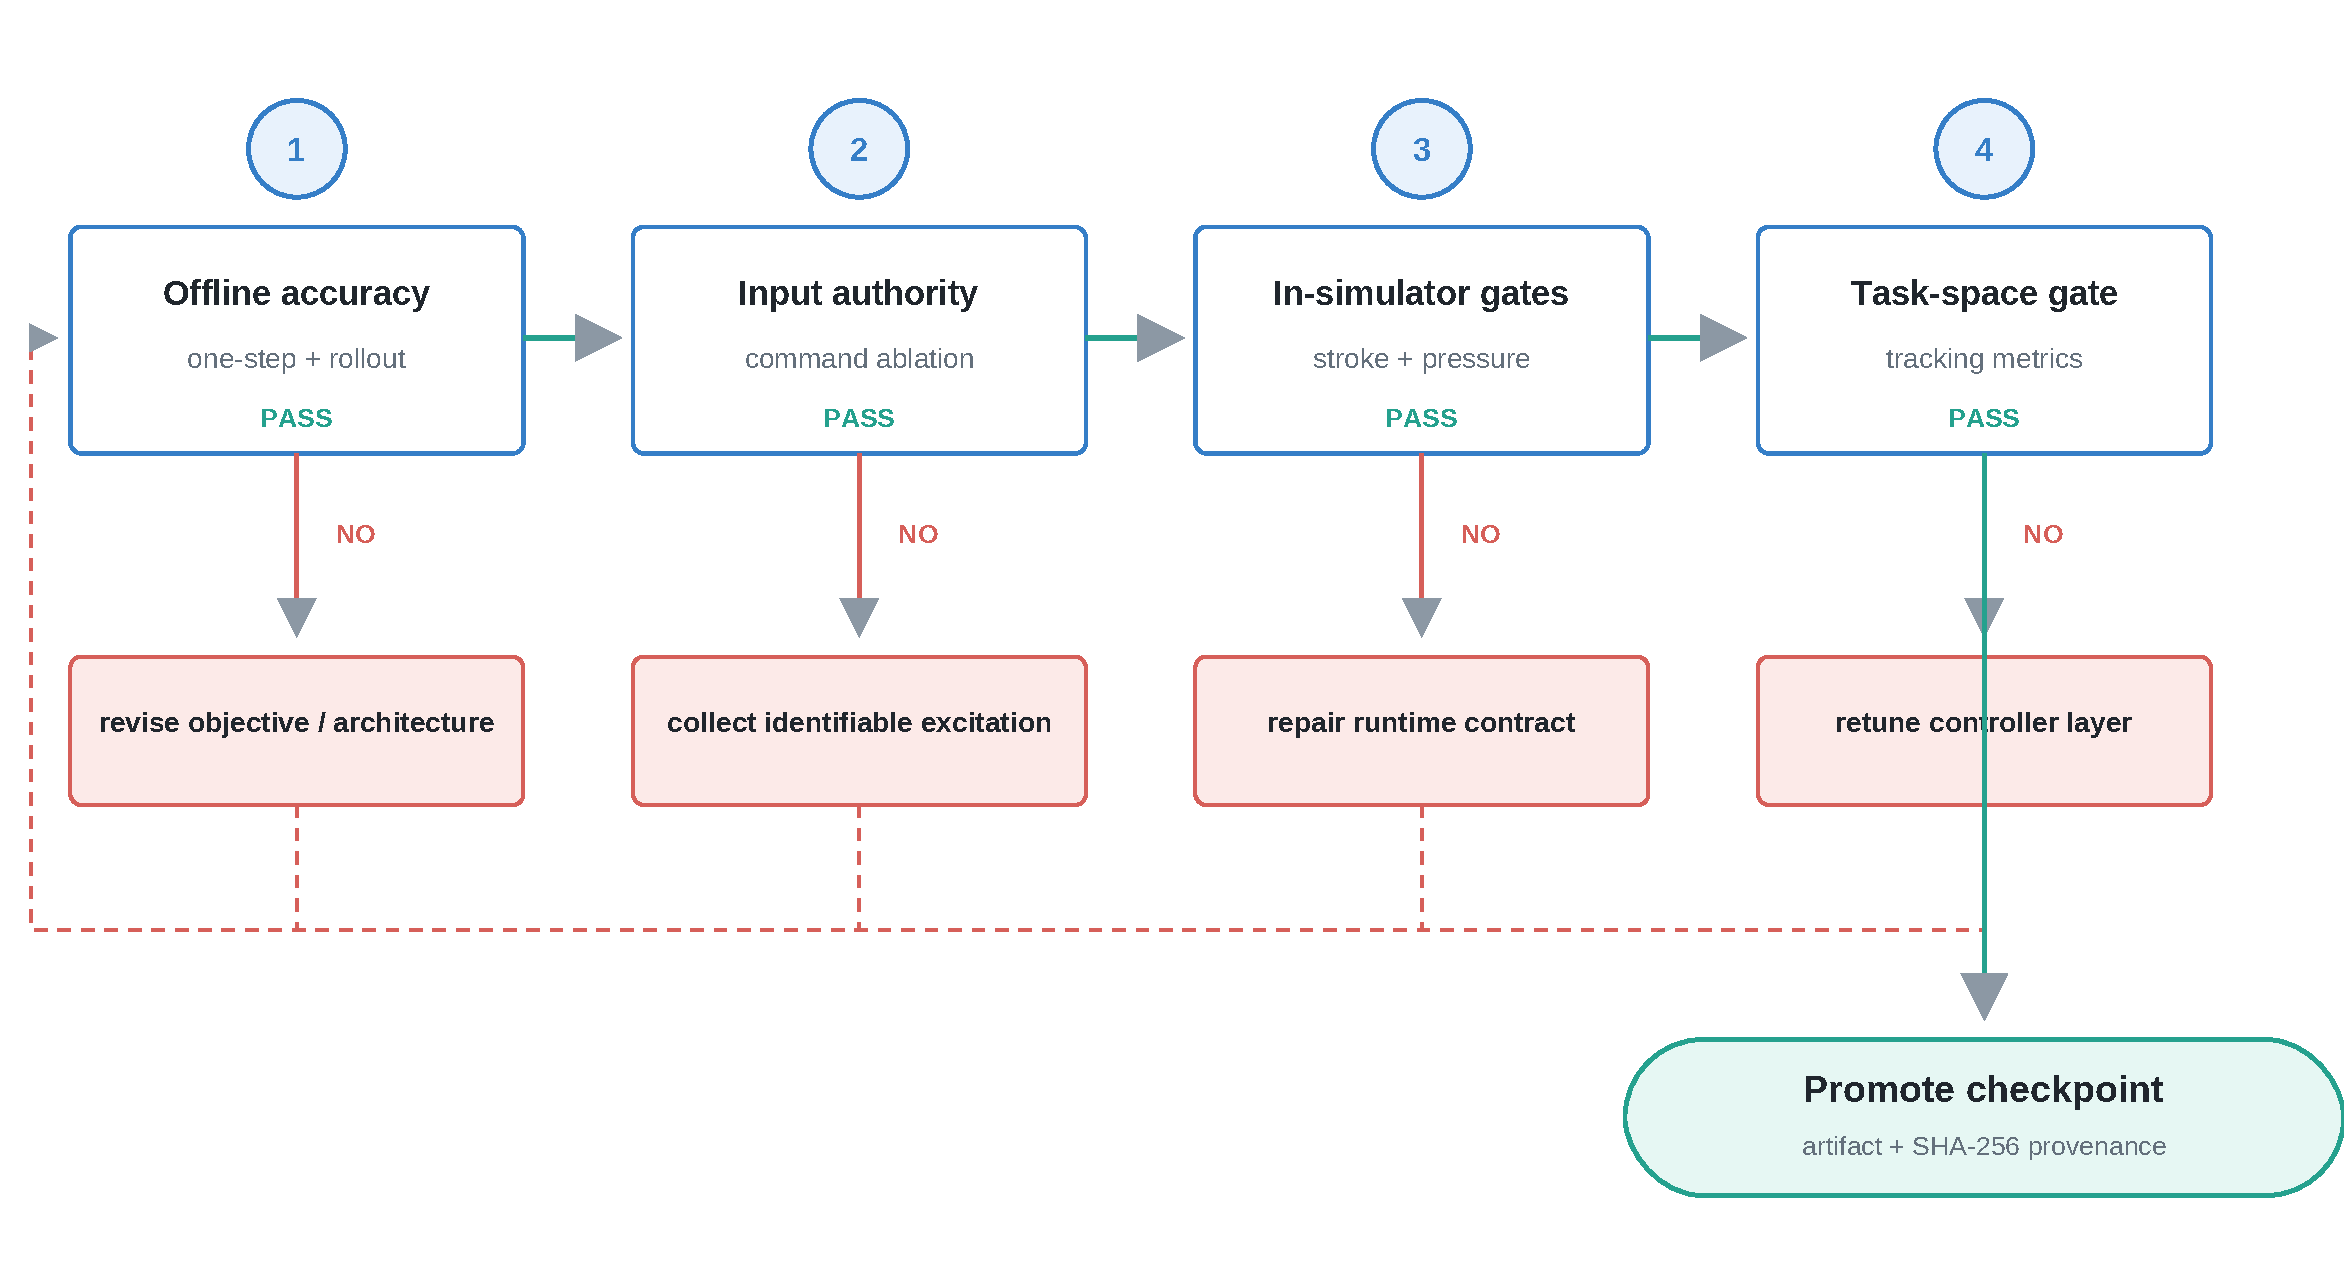
\includegraphics[width=.8\textwidth]{images/models_acceptance_flow}
  \caption{The acceptance ladder that every learned model in this
  thesis must climb before deployment. A candidate that fails a gate
  exits right into the corresponding repair loop and re-enters from the
  top; only a candidate that passes all four gates is promoted, and the
  promoted artifact is recorded together with its SHA-256 hash.}
  \label{fig:models:acceptance}
\end{figure}

%% ----- fig:models:nn-architectures -----
\begin{figure}[tb]
  \centering
  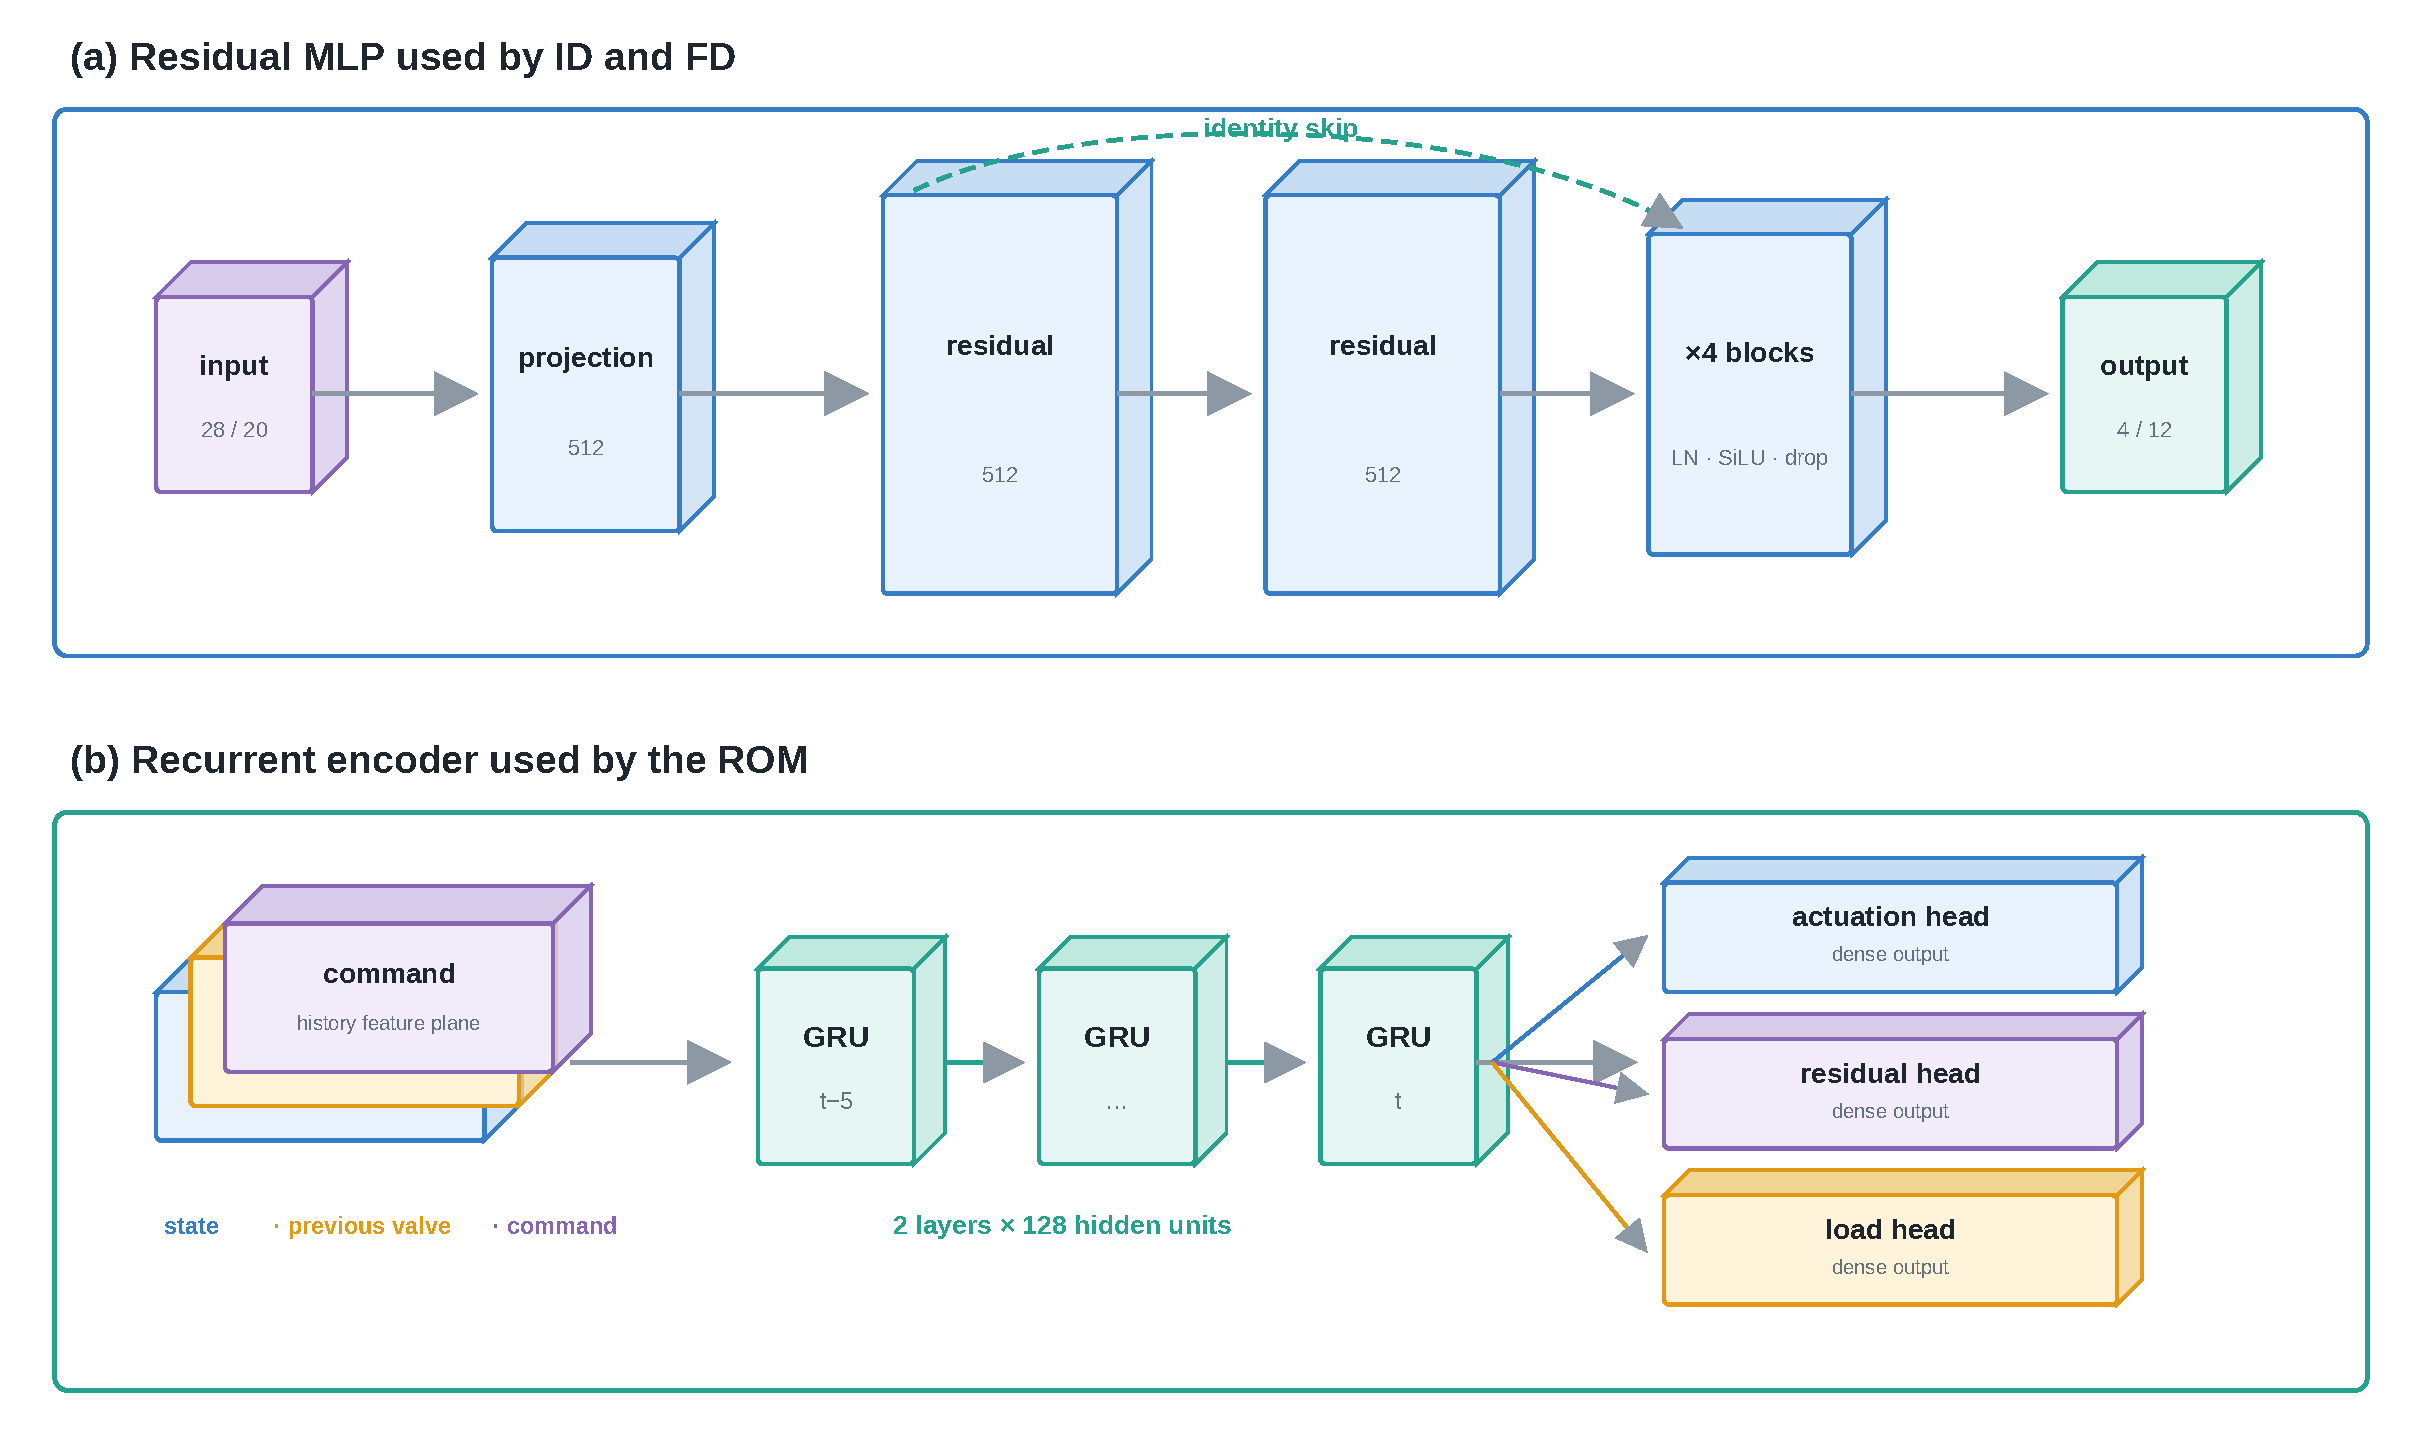
\includegraphics[width=\textwidth]{images/models_nn_architectures}
  \caption{The two network families used by the learned actuator
  models. (a)~The residual MLP trunk shared by the ID and FD networks:
  an input projection to width 512, four pre-activation residual blocks
  (Linear--LayerNorm--SiLU--Dropout--Linear with an identity skip), and
  a linear output head. Only the input and output widths differ between
  ID and FD. (b)~The ROM's recurrent encoder, unrolled over its six
  history steps: each step consumes the 24-D feature vector, the hidden
  state carries pressure and command transients across time, and the
  final latent $\bm{h}_k$ feeds the actuation, residual, and load
  heads.}
  \label{fig:models:nn-architectures}
\end{figure}

%% ----- fig:models:excitation -----
\begin{figure}[tb]
  \centering
  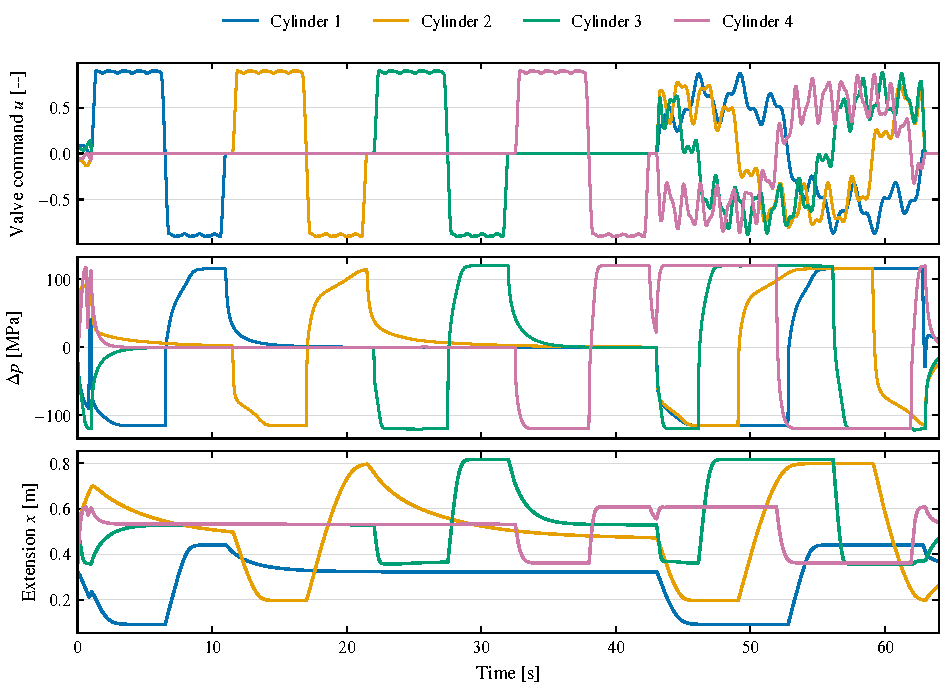
\includegraphics[width=\textwidth]{images/ch5_excitation_dataset}
  \caption{One run of the strict open-loop excitation dataset (nominal plant
  draw, $\unit[0.01]{s}$ sampling). Top: the rank-4 open-loop valve
  commands. The channels are excited individually in the first four segments
  and simultaneously in the final segment. Middle: resulting chamber
  pressure differences, including relief-limit episodes. Bottom: cylinder
  extension responses. The same excitation is repeated on three further
  randomized plant draws.}
  \label{fig:models:excitation}
\end{figure}

%% ----- fig:models:rom-training -----
\begin{figure}[tb]
  \centering
  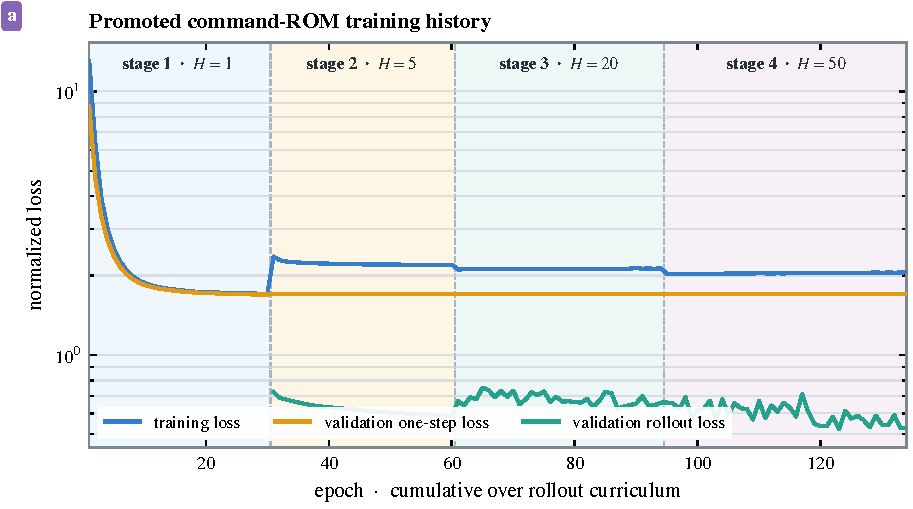
\includegraphics[width=\textwidth]{images/ch5_rom_training_history}
  \caption{Training history of the promoted command-ROM run over the
  four-stage rollout curriculum ($H$ is the recursive rollout horizon of
  each stage). The step in training loss at each stage boundary reflects
  the added longer-horizon rollout term; the validation one-step loss
  remains stable while the validation rollout loss continues to improve
  through stage~4.}
  \label{fig:models:rom-training}
\end{figure}

%% ----- tab:models:notation (folded into running prose) -----
\begin{table}[tb]
  \centering
  \caption{Cylinder-space notation used by all learned models.}
  \label{tab:models:notation}
  \begin{tabular}{llp{7.6cm}}
    \toprule
    Symbol & Dimension & Meaning \\
    \midrule
    $T$ & -- & learned-model sample time, $\unit[0.05]{s}$ \\
    $\bm{x}_k$, $\dot{\bm{x}}_k$ & $\mathbb{R}^4$ & cylinder extension [m] and extension velocity [m/s] \\
    $\Delta\bm{p}_k$ & $\mathbb{R}^4$ & chamber pressure difference [Pa] \\
    $\bm{F}_k$ & $\mathbb{R}^4$ & logged rod force [N] \\
    $\bm{u}_k$ & $[-1,1]^4$ & normalized proportional-valve command \\
    $\bm{c}_k = [\Delta\bm{x}^*_k, \Delta\dot{\bm{x}}^*_k]$ & $\mathbb{R}^8$ & desired extension and velocity increments \\
    $\Delta(\cdot)_k = (\cdot)_{k+1} - (\cdot)_k$ & -- & within-run one-step increment \\
    $\hat{(\cdot)}$ & -- & model prediction \\
    $\bm{h}_k$ & $\mathbb{R}^{128}$ & recurrent latent state of the ROM encoder \\
    \bottomrule
  \end{tabular}
\end{table}

%% ----- tab:models:fd-strict (numbers folded into running prose) -----
\begin{table}[tb]
  \centering
  \caption{Strict-excitation validation of the FD model before and after
  strict retraining. The valve-zero error ratio is the rollout RMSE with
  zeroed valve input divided by the RMSE with the true valve input at a
  $\unit[0.5]{s}$ horizon; a ratio near 1 means the model ignores the valve.}
  \label{tab:models:fd-strict}
  \begin{tabular}{lcc}
    \toprule
    Metric & Paired-control FD & Strict FD \\
    \midrule
    Valve-zero error ratio at $\unit[0.5]{s}$ & $\approx 0.94$ & $1.81$ \\
    Extension rollout RMSE at $\unit[0.5]{s}$ & $\unit[75.2]{mm}$ & $\unit[12.4]{mm}$ \\
    Extension rollout RMSE at $\unit[1.0]{s}$ & $\unit[157.9]{mm}$ & $\unit[27.3]{mm}$ \\
    One-step $\Delta x$ $R^2$ (per-axis range) & $-5.7$ to $0.60$ & $0.76$ to $0.98$ \\
    \bottomrule
  \end{tabular}
\end{table}
